\documentclass[tikz, border=10pt]{standalone}
\usepackage{tikz}
\usepackage[sfdefault]{roboto}
\usepackage[T1]{fontenc}
\usetikzlibrary{shapes.misc, positioning, arrows.meta, fit, calc, backgrounds}

\begin{document}

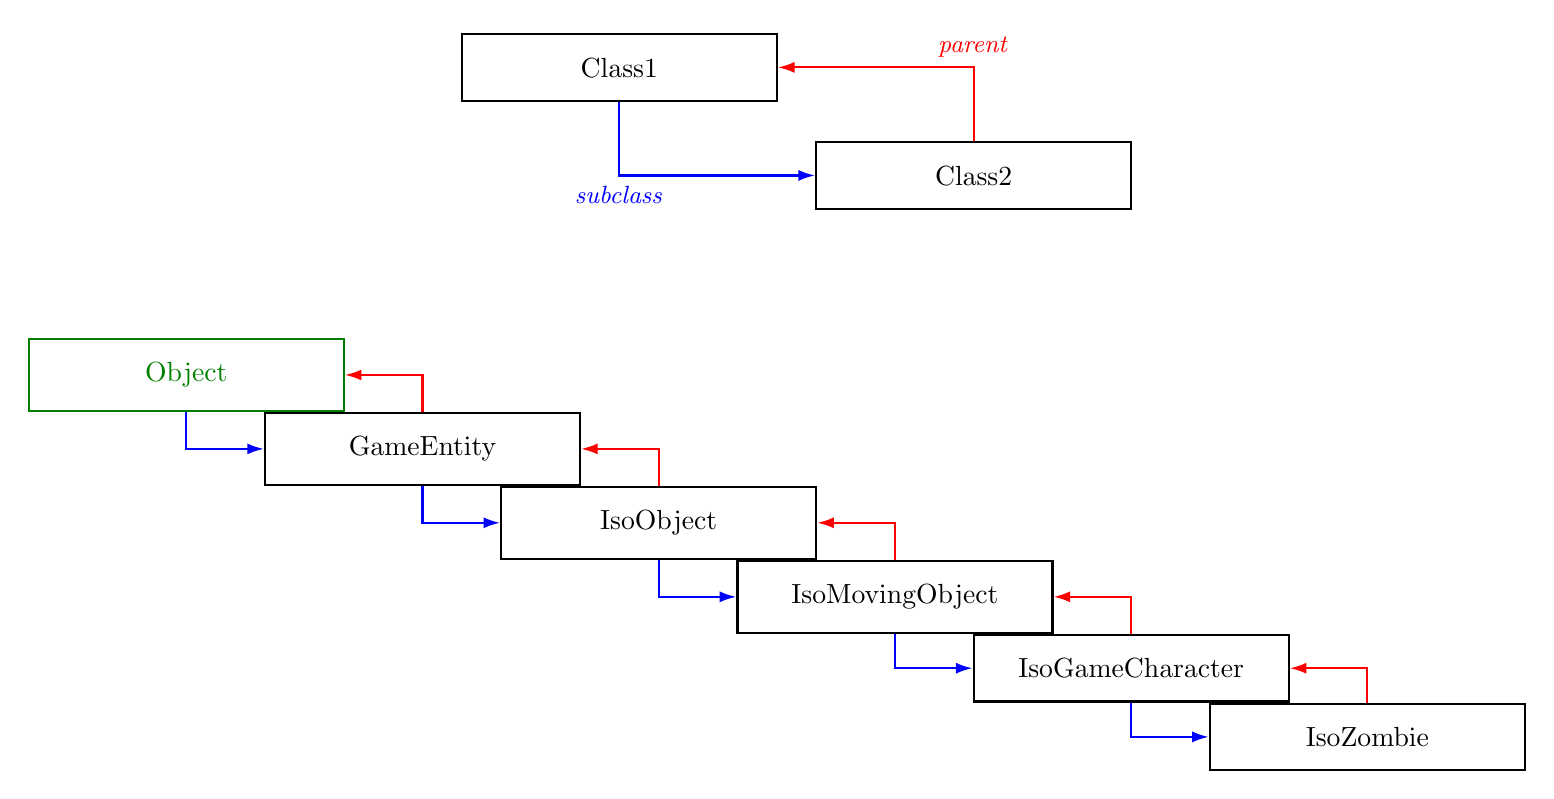
\begin{tikzpicture}[
    node distance=0.3cm,
    box/.style={rectangle, draw, thick, minimum width=4cm, inner sep=0.3cm},
    func/.style={font=\ttfamily\small, inner sep=0.15cm},
    arrow/.style={-{Latex[length=6pt, width=4pt]}, thick},
    dashed_arrow/.style={-{Latex[length=6pt, width=4pt]}, thick, dashed},
    line/.style={thick},
]

%% MAIN LOGIC
    % original tools
    \node[box] (parent) {Class1};
    \node[box, below=0.5cm of parent, xshift=4.5cm] (child) {Class2};

    \draw[arrow, color=blue] (parent.south) |- node[below, font=\small] {\textit{subclass}} (child.west);
    \draw[arrow, color=red] (child.north) |- node[above, font=\small] {\textit{parent}} (parent.east);

%% EXAMPLE
    \node[box, below=3cm of parent,           xshift=-5.5cm, color=green!50!black] (object) {Object};
    \node[box, below=0cm of object,           xshift=3cm] (gameentity) {GameEntity};
    \node[box, below=0cm of gameentity,       xshift=3cm] (isoobject) {IsoObject};
    \node[box, below=0cm of isoobject,        xshift=3cm] (isomovingobject) {IsoMovingObject};
    \node[box, below=0cm of isomovingobject,  xshift=3cm] (isogamecharacter) {IsoGameCharacter};
    \node[box, below=0cm of isogamecharacter, xshift=3cm] (isozombie) {IsoZombie};

    \draw[arrow, color=blue] (object.south) |- (gameentity.west);
    \draw[arrow, color=blue] (gameentity.south) |- (isoobject.west);
    \draw[arrow, color=blue] (isoobject.south) |- (isomovingobject.west);
    \draw[arrow, color=blue] (isomovingobject.south) |- (isogamecharacter.west);
    \draw[arrow, color=blue] (isogamecharacter.south) |- (isozombie.west);

    \draw[arrow, color=red] (isozombie.north) |- (isogamecharacter.east);
    \draw[arrow, color=red] (isogamecharacter.north) |- (isomovingobject.east);
    \draw[arrow, color=red] (isomovingobject.north) |- (isoobject.east);
    \draw[arrow, color=red] (isoobject.north) |- (gameentity.east);
    \draw[arrow, color=red] (gameentity.north) |- (object.east);



\end{tikzpicture}

\end{document}
